\chapter{Introduction}
\label{sec:introduction}

Finding the shortest path between a vertex pair in a graph is one
of the most fundamental computational graph problems. Papers like
Dijkstra\cite{Dijkstra59anote} and Bellman-Ford\cite{bellman} presents
algorithms able to determine the shortest path for a single vertex pair, but
these algorithms does not scale well, as they need to visit every vertex in
the graph to come up with a result. Thus, these algorithms are a poor choice
for applications that needs to answer shortest path queries for large graphs
extremely fast.

Now suppose you are given a connected weighted undirected graph $G=(V,E)$
consisting of $n$ vertices and $m$ edges, and you are asked to come up with a
solution able to answer shortest path queries extremely fast.

The naive solution is to compute the shortest path between every vertex pair
$(u,v) \in V \times V$ and store the information in a lookup table using
$(u,v)$ as key for the entry. Subsequent distance queries can be answered in
constant time simply by performing a lookup in the hash table.
However, there are strong objections to this naive solution.

First of all the preprocessing time may simply be too long, and secondly,
even if one is willing to wait for the preprocessing to finish, the size of
the final lookup table may be too large to store efficiently. Using Thorups
shortest path algorithm for undirected graphs\cite{thorupsssp}, which offers
$O(m)$ time complexity, to compute the distances from each vertex $v\in V$,
one gets a time complexity of $O(nm)$ while $O(n^2)$ space is required by the
lookup table.

If one can settle for approximated distances instead of exact ones,
approximate distance oracles is the better alternative for undirected
graphs. Approximate distance oracles is a data structure presented by Thorup
and Zwick\cite{tu}, it offers much better space and construction time
complexities, while still being able to answer shortest path queries in
constant time.

More precisely the paper describe for any integer $k \leq 1$, a preprocessing
algorithm that runs $O(kmn^{1/k})$, producing a data structure of size
$O(kn^{1+1/k})$. The data structure can return approximate distances of a
finite stretch $t$. An estimated distance $\hat{\delta}(u,v)$ from $u$ to $v$
is said to be within the stretch $t$ if and only if $\delta(u,v)\leq
\hat{\delta}(u,v)\leq t \cdot\delta(u,v)$ where $\delta(u,v)$ denotes the
exact shortest distance. The actual stretch of the produced estimates is
at most $2k-1$, but it may be as low as $1$. Thorup and Zwick does not discuss
this further.

In this report I study - through experiments - the average actual stretch of
distances produced by \emph{Stretch-3} ($k=2$) approximate distance oracles. A
high quality implementation of the algorithm has been developed to conduct
the experiments, and has been used to compute approximate distance oracle
data structures for graphs representing internet topologies and road networks.

Using a sample of vertex pairs from each graph, and comparing the actual
shortest path against the approximated shortest path in the sample, I show the
average actual stretch for these internet topologies and road networks. The
goal is to provide data that indicates what actual stretch to expect, if you
apply approximate distance oracles to these classes of graphs.

The rest of the article is organized as follows: In the next short chapter I
introduce some basic background material. Then, \autoref{sec:ado} presents an
introduction to approximate distance oracles. In \autoref{sec:implementation}
I discuss obstacles and solution regarding the implementation and development
process. Finally in \autoref{sec:experiments} I conduct and discuss my
experiments before I present my conclusions in \autoref{sec:conclusion}.




\section{Lets talk a bit about routing}

\begin{frame}[fragile]
  \frametitle{Routing Scheme}
    A routing scheme is a distributed algorithm that allows any
    source node to route messages to any destination node, given
    destination node's name

    \begin{description}
        \item[Input] a network $G$ (a weighted connected graph)
        \item[Output] a routing scheme for G
    \end{description}
\end{frame}

\begin{frame}{XY-routing}
  \begin{figure}
    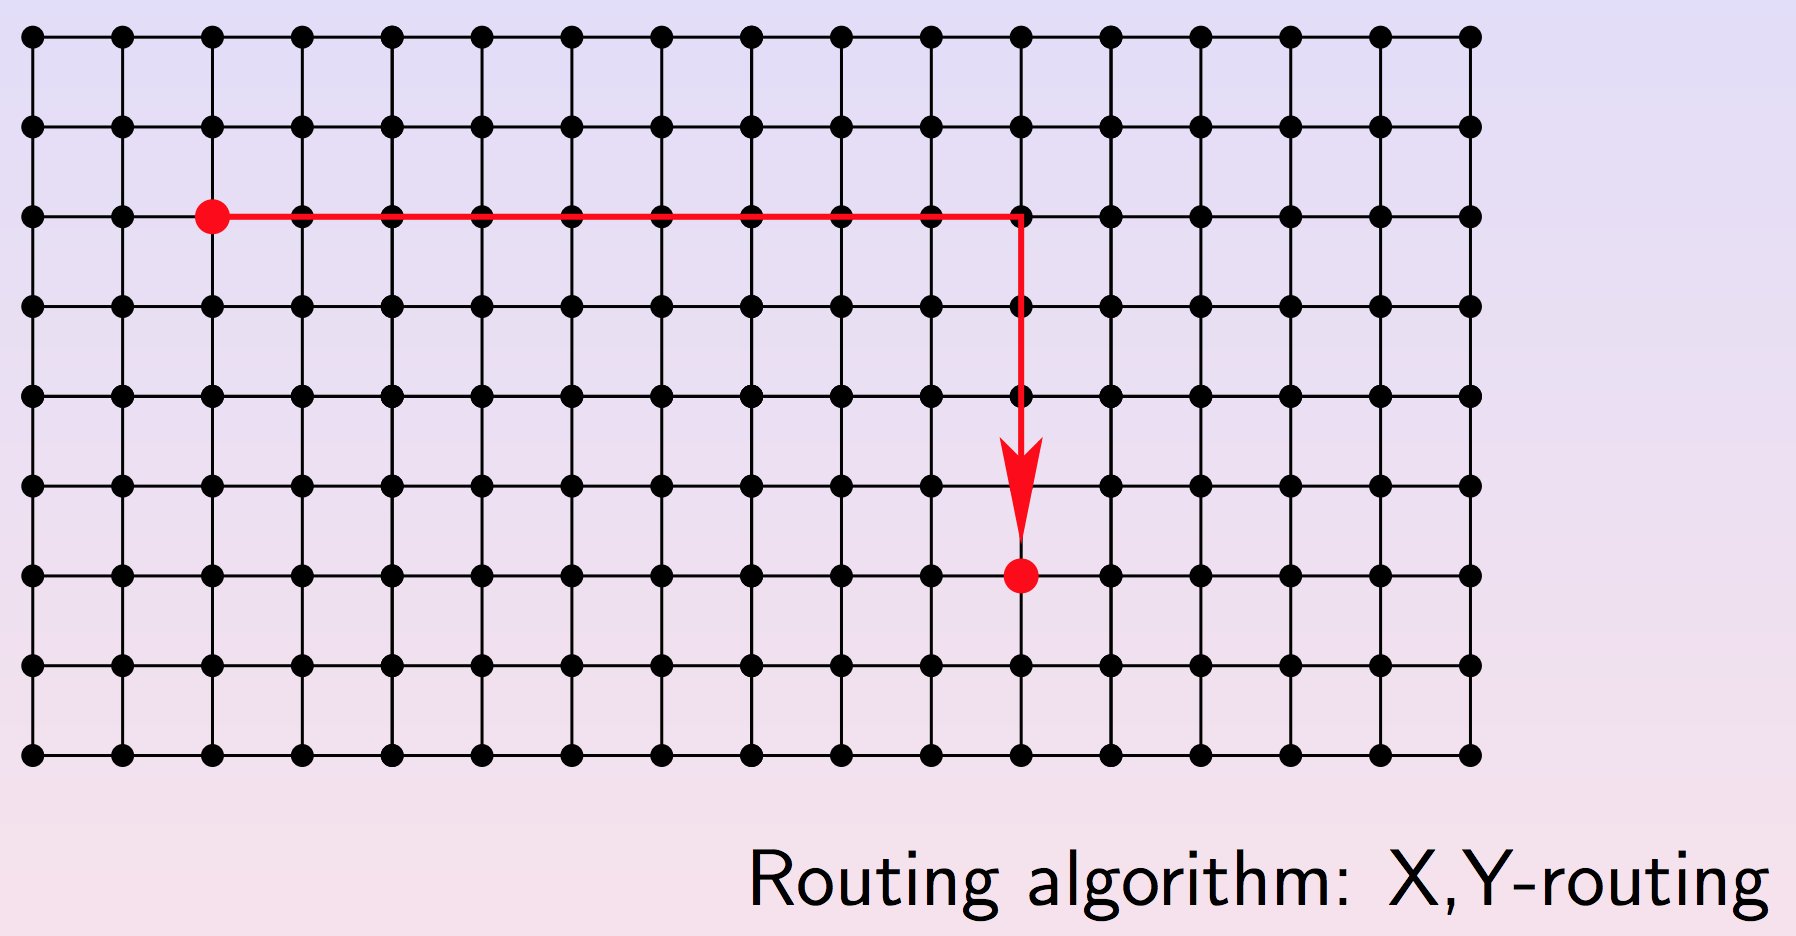
\includegraphics[scale=0.3]{images/xyrouting.png} 
  \end{figure}
\end{frame}

\begin{frame}[fragile]
  \frametitle{Routing Scheme}
     
  \begin{block}{Example: Trivial routing on min cost paths}
      \begin{itemize}
        \item On each node, for each of the possible $(n-1)$ destinations,
        store a port number leading to the next node on a min cost path to the
        destination.
        \item Requires each node to store $\Omega (n\; log\; n)$ bits.
        \item Does not scale very well.
      \end{itemize}
  \end{block}
\end{frame}

\begin{frame}[fragile]
  \frametitle{Minimizing parameters}
  When working with routing, two factors are normally of interest:
  \begin{description}
    \item[Stretch] The max ratio over all source-destination pairs between the
        cost of the path taken by the routing scheme and the cost of a min
        cost path.
    \item[Memory] The max number of bits over all nodes stored for the routing
        scheme. (ballanced is preferred)
  \end{description}
\end{frame}

\begin{frame}[fragile]
  \frametitle{Labeled Routing or Name-Independent Routing}

  In labeled routing we can choose a label for each vertex.
  Lets use coordinates. Now we can easily route. If an aversery
  label the vertices randomly, routing gets harder.

  \begin{figure}
    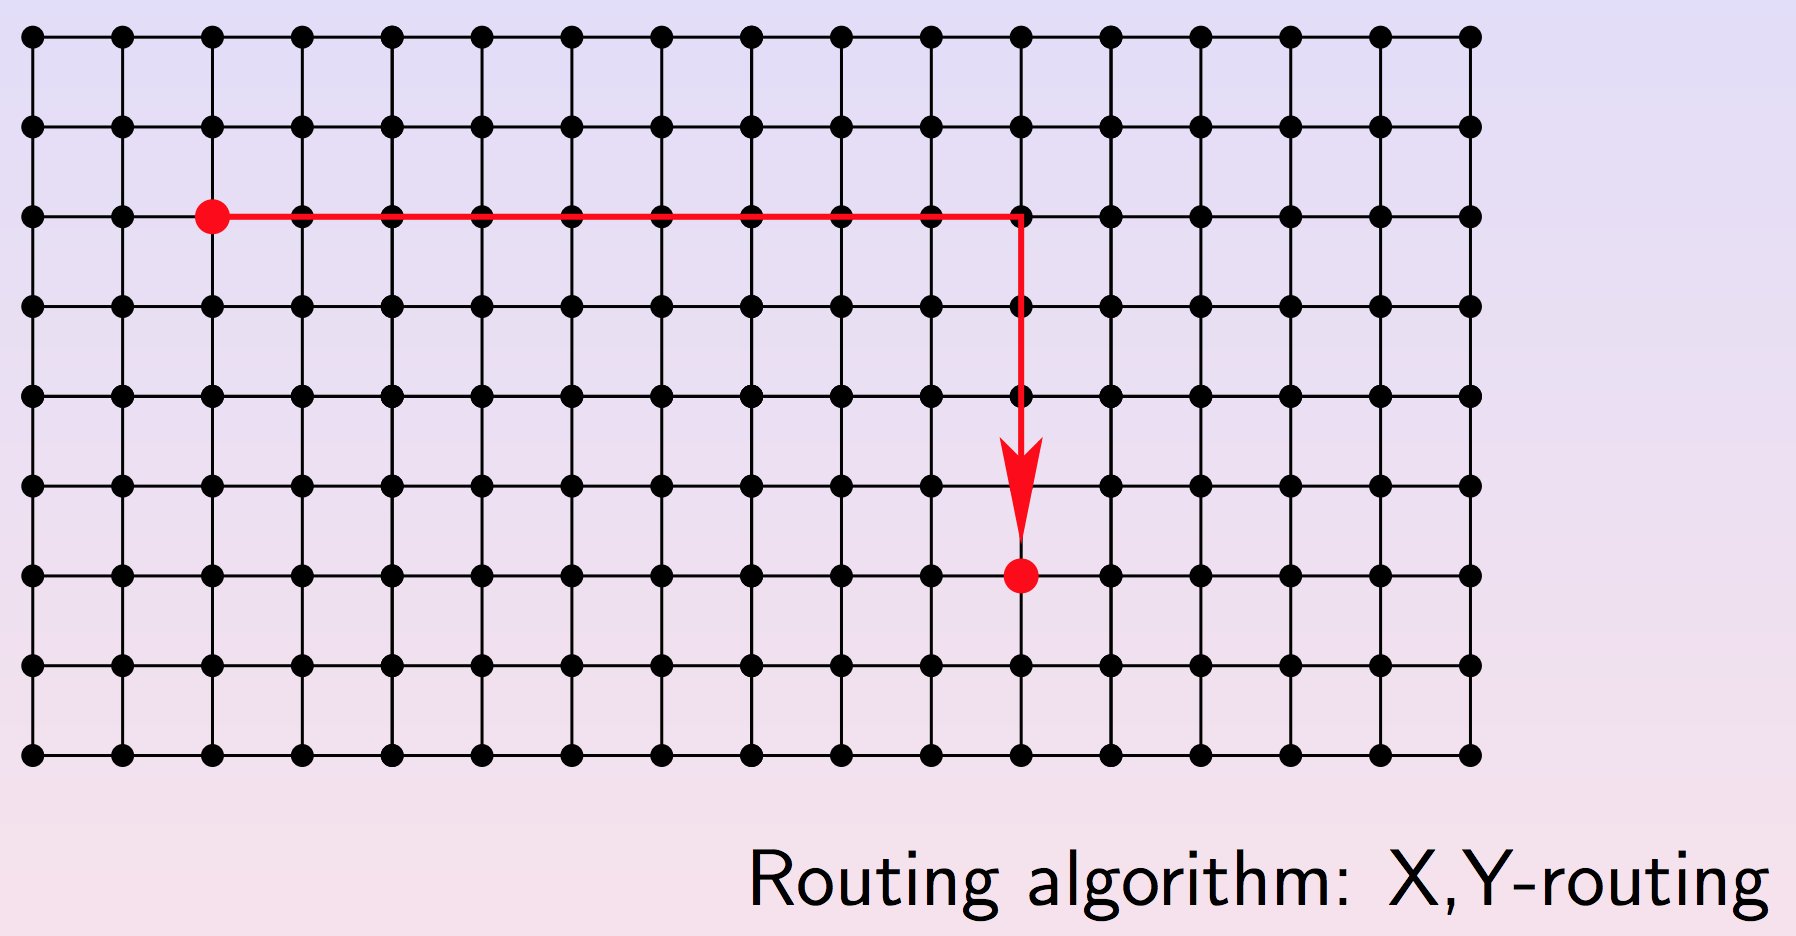
\includegraphics[scale=0.3]{images/xyrouting.png} 
  \end{figure}
\end{frame}

